%\vspace{-0.25in}
\section{Experiments}
%\vspace{-0.05in}
\subsection{2D regression}\label{sect:syn}
\vspace{-0.05in}
For evaluation, we first examined the proposed approach in two synthetic benchmark tests, namely, meta learning of \textit{CosMixture} and \textit{Alpine} functions ({\url{http://infinity77.net/global_optimization/test_functions.html}}), both of which are 2D regression tasks. We considered two families of tasks. In the first family, each task aims to learn a specific \textit{CosMixture} function of the following form,
\begin{align}
	f_1(\x) = -0.1 \sum\nolimits_{i=1}^d A \cos(\omega x_i + \phi) - \sum\nolimits_{i=1}^d x_i^2,
\end{align}
where $\x \in [-1, 1]^2$, $d =2$, $A \in [0.1, 1.0]$, $\omega \in [0.5 \pi, 2.0\pi]$, and $\phi \in [3.0, 6.0]$. 
The second family of tasks learn instances of the \textit{Alpine} function,  
\begin{align}
	f_2(\x) = \sum\nolimits_{i=1}^d |x_i \sin(x_i + \phi_i) + 0.1x_i|,
\end{align}
where $\x \in [10, 10]^2$, $d=2$, $\phi_1 \in [-\frac{5}{12}\pi, \frac{5}{12}\pi]$, and $\phi_2 \in [-\frac{5}{12}\pi, \frac{5}{12}\pi]$.   An instance of each function is shown in Fig. \ref{fig:CosMixture-ins} and \ref{fig:Alpine-ins}. The learning model for both task populations is a neural network with two hidden layers, each consisting of 32 neurons with  Tanh activation. %Each hidden layer includes $32$ neurons. 
To conduct meta-learning for each task population, we randomly sampled $100$ tasks, where for each task, the parameters of the target function, \ie $\{A, \omega, \phi\}$ in \textit{CosMixture} and $\{\phi_1, \phi_2\}$ in \textit{Alpine}, are uniformly sampled from their ranges. We considered two meta-learning settings: 50shot-50val, where we used 50 examples for meta-training and 50 another examples in meta-validation, and 100shot-100val, where both the meta-training and meta-validation losses employed 100 examples.  These examples are non-overlapping and generated by uniformly sampling from the input domain. Given the learned initialization, we tested on $100$ new tasks, where the task training data were generated in the same way as in the meta-training and $100$ another examples were sampled to evaluate the prediction accuracy. 

\begin{figure*}[t]
	\centering
	\setlength\tabcolsep{0.01pt}
	\captionsetup[subfigure]{aboveskip=0pt,belowskip=0pt}
	\begin{tabular}[c]{ccc}
		\begin{subfigure}[t]{0.32\textwidth}
			\centering
			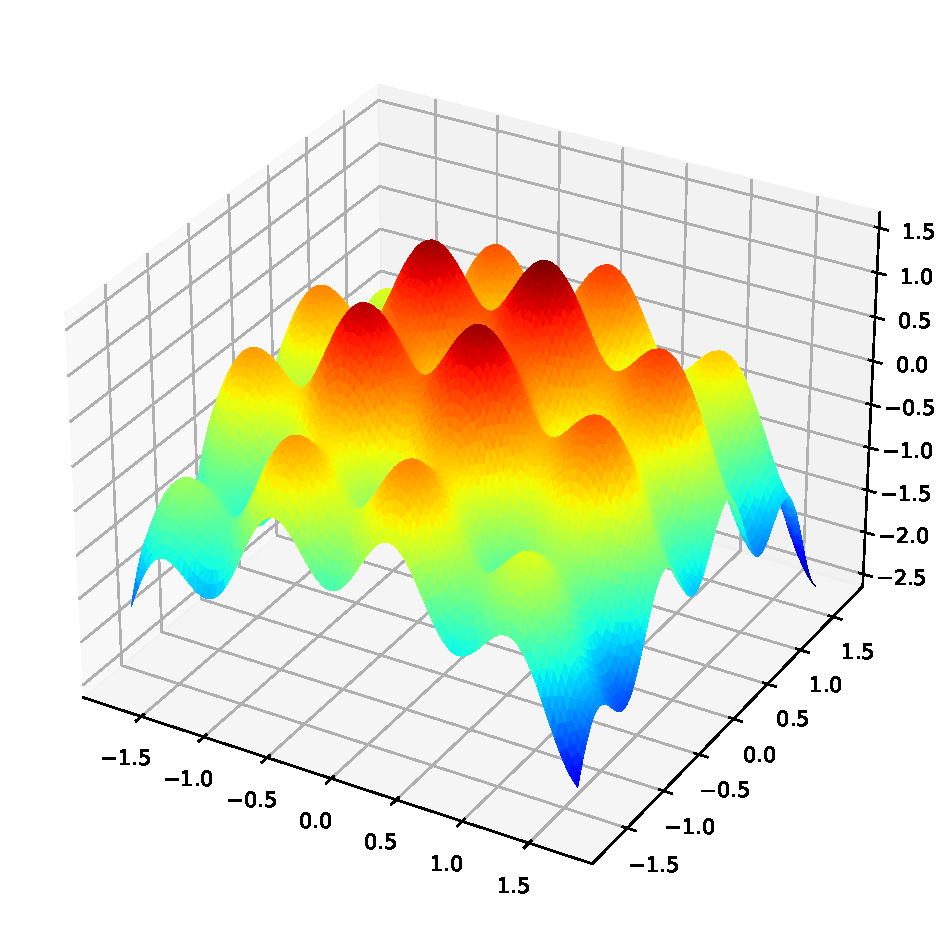
\includegraphics[width=\textwidth]{./figs/CosMixture2D.pdf}
			\caption{\small \textit{CosMixture} instance} \label{fig:CosMixture-ins}
		\end{subfigure} 
		&
		\begin{subfigure}[t]{0.32\textwidth}
			\centering
			\includegraphics[width=\textwidth]{./figs/new/CosMixture2D-50shot-50query-200inners-eps-converted-to.pdf}
			\caption{\small \textit{CosMixture}: 50shot-50val}
		\end{subfigure} 
		&
		\begin{subfigure}[t]{0.32\textwidth}
			\centering
			\includegraphics[width=\textwidth]{./figs/new/CosMixture2D-100shot-100query-500inners-eps-converted-to.pdf}
			\caption{\small \textit{CosMixture}: 100shot-100val}
		\end{subfigure} 	\\
		\begin{subfigure}[t]{0.32\textwidth}
			\centering
			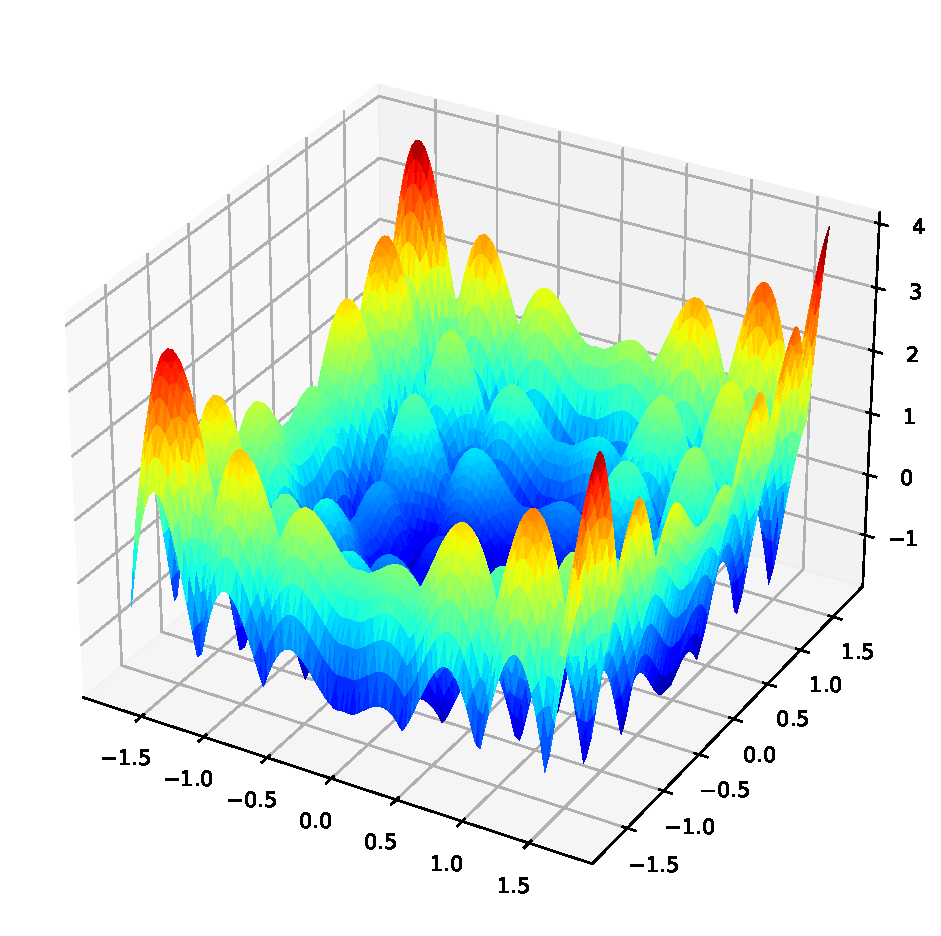
\includegraphics[width=\textwidth]{./figs/Alpine2D.pdf}
			\caption{\small \textit{Alpine} instance} \label{fig:Alpine-ins}
		\end{subfigure} 
		&
		\begin{subfigure}[t]{0.32\textwidth}
			\centering
			\includegraphics[width=\textwidth]{./figs/new/Alpine2D-50shot-50query-200inners-eps-converted-to.pdf}
			\caption{\small \textit{Alpine}: 50shot-50val}
		\end{subfigure} 
		&
		\begin{subfigure}[t]{0.32\textwidth}
			\centering
			\includegraphics[width=\textwidth]{./figs/new/Alpine2D-100shot-100query-500inners-eps-converted-to.pdf}
			\caption{\small \textit{Alpine}: 100shot-100val}
		\end{subfigure} 
	\end{tabular}
	%	\vspace{-0.1in}
	\caption{\small Prediction error of the neural network in learning \textit{CosMixture} and \textit{Alpine} function families, starting from the initialization provided by different meta-learning approaches. (a,d) are the instances of the two types of functions. 50shot-50val means 50 examples were used for meta-training and another 50 examples for meta-validation. 100shot-100val means both the meta-training and meta-validation used  100 examples. The results were averaged over 100 test tasks. } 	
	\label{fig:synthetic}
	\vspace{-0.1in}
\end{figure*}

\cmt{
\begin{figure*}[t]
	\centering
	\setlength\tabcolsep{0pt}
	\captionsetup[subfigure]{aboveskip=0pt,belowskip=0pt}
	\begin{tabular}[c]{cccc}
		\begin{subfigure}[t]{0.25\textwidth}
			\centering
			\includegraphics[width=\textwidth]{./figs/icml22/CosMixture2D-50shot-50query-200inners-trim.pdf}
			\caption{\small{ \textit{CosMixture}: 50shot-50val}}
		\end{subfigure} 
		&
	\begin{subfigure}[t]{0.25\textwidth}
		\centering
		\includegraphics[width=\textwidth]{./figs/icml22/Alpine2D-50shot-50query-200inners-trim.pdf}
		\caption{\small \textit{Alpine}: 50shot-50val}
	\end{subfigure}
		&
		\begin{subfigure}[t]{0.25\textwidth}
			\centering
			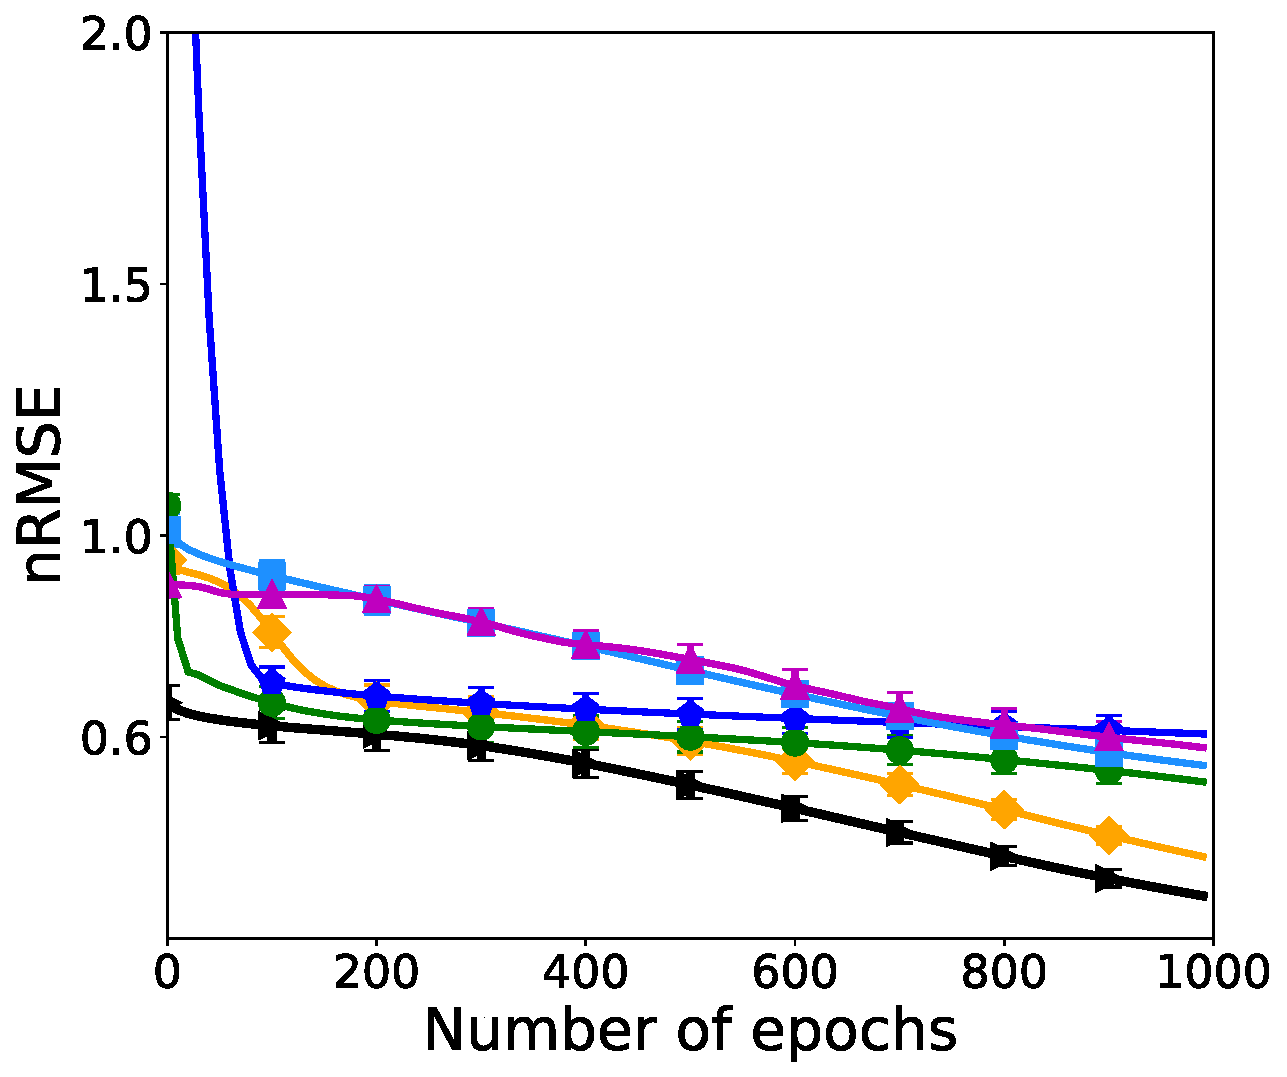
\includegraphics[width=\textwidth]{./figs/icml22/CosMixture2D-100shot-100query-500inners-trim.pdf}
			\caption{\small \textit{CosMixture}: 100shot-100val}
		\end{subfigure}  
		&
		\begin{subfigure}[t]{0.25\textwidth}
			\centering
			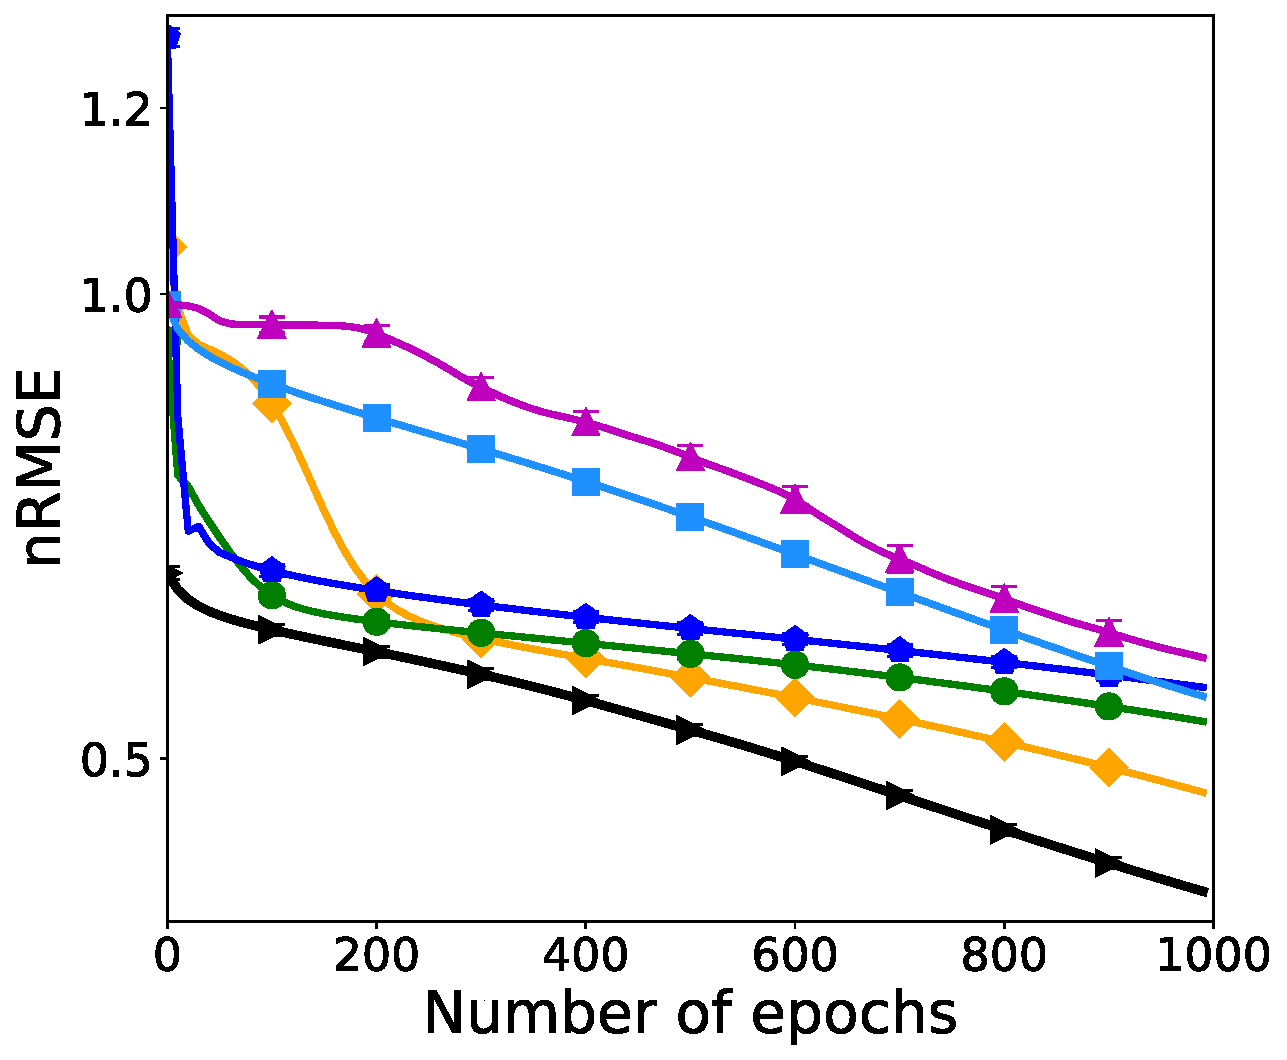
\includegraphics[width=\textwidth]{./figs/icml22/Alpine2D-100shot-100query-500inners-trim.pdf}
			\caption{\small \textit{Alpine}: 100shot-100val}
		\end{subfigure} 
	\end{tabular}
	\vspace{-0.1in}
	\caption{\small Prediction error of the neural network in learning \textit{CosMixture} and \textit{Alpine} function families, starting from the initialization provided by different meta-learning approaches.  50shot-50val means 50 examples were used for meta-training and another 50 examples for meta-validation. 100shot-100val means both the meta-training and meta-validation used  100 examples. The results were averaged over 100 test tasks. } 	
	\label{fig:synthetic}
%	\vspace{-0.1in}
\end{figure*}
}

\noindent \textbf{Competing Methods.} To examine the effectiveness of our method \ours, \cmt{in computing the gradient in optimization based meta-learning,} we tested the following MAML based approaches for an \textit{apples-to-apples} comparison: (1) the original \maml~\citep{finn2017model}, (2) First-order \maml (\fomaml)~\citep{finn2017model}, which ignores the Jacobian in the gradient computation and uses the gradient \cmt{of the meta-validation loss} w.r.t. the trained parameters to update the initialization, (3) \rap~\citep{nichol2018first}, which subtracts the gradient w.r.t. the trained parameter by the current initialization as the updating direction, (4) Implicit \maml (\imaml)~\citep{rajeswaran2019meta}, which introduces a proximal regularizer in the meta-training loss, and uses conjugate gradient to compute the gradient w.r.t. the initialization. 

All the methods were implemented with PyTorch~\citep{paszke2019pytorch}. For \maml, we used a high-quality open source implementation ({\url{https://github.com/dragen1860/MAML-Pytorch}}); for \imaml, we used the  implementation of the original authors ({\url{https://github.com/aravindr93/imaml_dev}}). For our approach \ours, we used the Torchdiffeq library ({\url{https://github.com/rtqichen/torchdiffeq}}) to accomplish ODE solving with RK45. In the inner optimization, all the competing methods used the standard gradient descent (GD) with step size $\alpha = 0.01$. For \imaml, the strength of the proximal regularizer was chosen as $\lambda=1$ \cmt{\footnote{We also tested with other choices, \eg $0.5$ or $2$ as used in the original paper~\citep{rajeswaran2019meta}. The performance was almost the same.}} and 5 CG steps were conducted for Newton-CG optimization.  For our method, we used the same step size (\ie $0.01$) to run modified Euler's method~\citep{ascher1998computer} for solving the adjoint ODE. 
In the outer optimization, all the methods used the ADAM algorithm~\citep{kingma2014adam}, and the learning rate was set to $10^{-3}$. Each time, a mini-batch of five tasks were sampled to conduct inner-optimization, and then update the initialization in the outer-level. We ran $5,000$ meta-epochs for each method.  For the 50shot-50val setting, we ran $200$ GD steps for \fomaml, \rap, \imaml, and for our method \ours, set $T=2$ (that corresponds to 200 GD steps with $\alpha=0.01$). For the 100shot-100val setting, we ran 500 GD steps for \fomaml, \rap, \imaml, and set $T=5$ for \ours accordingly. By contrast, \maml ran $20$ and $50$ GD steps, respectively. Note that \maml cannot run too many GD steps without exhausting computational memory (see Section \ref{sect:memory}). We also evaluated \maml with only one GD step (the most common choice) for both settings; we denote such results by \maml-1. \zsdc{At the adaptation stage (meta-test), we ran the same number of GD steps with the initialization learned by every method:  200 steps for 50shot-50val and 500 steps for 100shot-100val, with the same step size as in the meta training.}
We executed all the algorithms  on a Linux workstation with an NVIDIA GeForce RTX 3090 GPU card that includes $24$ GB of G6X memory. 

In Fig. \ref{fig:synthetic}b,c, e and f, we show that starting with the learned initialization of each method, how the prediction error of the NN model on the test tasks varies along with the increase of training epochs.   The prediction error for each task is computed as the normalized root-mean-square error (nRMSE). We averaged the nRMSE over the $100$ test tasks and report the standard deviation. As we can see, in all the cases, our approach, \ours, always finds the initialization that leads to the best learning progress and performance  --- the NN models exhibit smaller prediction error throughout the training, as compared with using the initialization from the competing methods. \maml-1 is in general worse than \maml; the discrepancy is particularly evident for learning \textit{Alpine} functions with the 100shot-100val setting (see Fig. \ref{fig:synthetic}f). It implies that only performing one step GD in the inner-optimization might not properly reflect the quality of the initialization in training. Although \fomaml and \rap can run many GD steps, their performance is often worse than \maml, especially \rap, which is nearly always inferior to \maml. Such relatively poor performance might be attributed to the use of incorrect gradient information to update the initialization in these approaches. \imaml performed the second best at the beginning, but it was often surpassed by \maml or \fomaml after considerable training epochs. This might be due to (1) the proximity regularizer in the meta-training was not used in the actual training, which introduces some inconsistency, and (2) the inner optimization (though with 200/500 GD steps) has yet to achieve the optimum, and so the obtained gradient w.r.t. the initialization is still inaccurate. \zsdc{Note that the nRMSE for 100shot-100val seems a bit higher than 50shot-50val at the early stage, which might because the former involves a double quantity of examples, hence needs more epochs to train better and exhibits  slower learning progress.} Together these results have demonstrated the advantage of our method in being able to accurately compute the gradient for long inner-optimization trajectories. 

\vspace{-0.05in}
\subsection{Memory Consumption and Running Time}\label{sect:memory}
\vspace{-0.1in}
Next we examined the efficiency of our method in terms of memory usage and computational speed. To this end, we tested the 100shot-100validation setting in the meta learning of \textit{CosMinxture} functions. We varied the number of inner GD steps (with the step size $\alpha = 0.01$) for the competing approaches and the corresponding time ranges $[0, T]$ for ODEs in \ours. The average memory usage and running time are reported in Fig. \ref{fig:mem-usage} and \ref{fig:speed}, respectively. 
\begin{figure}[!htb]
	\centering
	\includegraphics[width=0.45\textwidth]{./figs/icml22/nGPU-eps-converted-to.pdf}
	\caption{\small Normalized GPU usage in meta learning of \textit{CosMixutre} with 100shot-100validation. The dashed line indicates the capacity of available GPU memory.}
	\label{fig:mem-usage}
	\vspace{-0.1in}
\end{figure}

\begin{figure}[!htb]
	\centering
	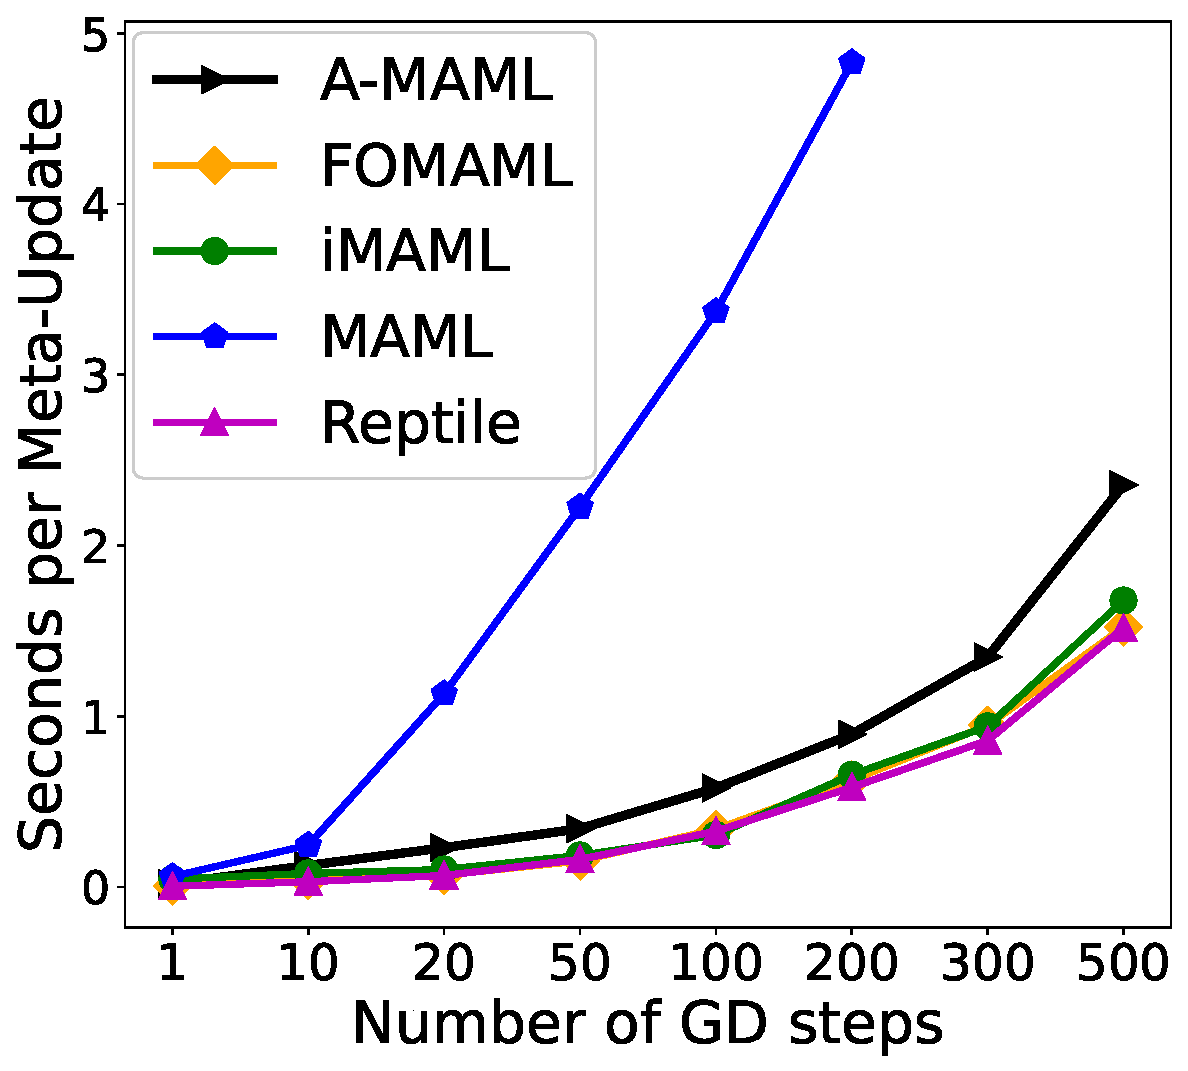
\includegraphics[width=0.45\textwidth]{./figs/icml22/speed-eps-converted-to.pdf}
	\caption{\small Running time of the inner gradient descent for \textit{CosMixutre}.}
	\label{fig:speed}
	%\vspace{-0.1in}
\end{figure}
\cmt{
%\setlength{\columnsep}{5pt}
%\begin{wrapfigure}{r}{0.5\textwidth}
\begin{figure}
	%	\vspace{-0.05in}
	\centering
	\setlength{\tabcolsep}{0pt}
	\begin{tabular}[c]{c}
		\begin{subfigure}[b]{0.25\textwidth}
			\centering
			\includegraphics[width=\linewidth]{./figs/icml22/nGPU.eps}
			\caption{}
		\end{subfigure} \\
		\begin{subfigure}[b]{0.235\textwidth}
			\centering
			\includegraphics[width=\linewidth]{./figs/icml22/speed.eps}
			\caption{} 
		\end{subfigure} 
	\end{tabular}
	%\vspace{-0.2in}
	\caption{\small Normalized GPU usage (a) and running time (b) in meta learning of \textit{CosMixutre} with 100shot-100validation.The dashed line in (a) indicates the capacity of available GPU memory.}
	\vspace{-0.1in}
	\label{fig:efficiency}
%\end{wrapfigure}
\end{figure}
}

As shown in Fig. \ref{fig:mem-usage}, \maml always occupies the most memory. With the increase of GD steps, its memory consumption grows exponentially. When \maml runs 200 inner GD steps, the memory is completely exhausted.  The result shows the creation and expansion of the computation graphs is very costly. By contrast,  \ours can accurately compute the gradient in a much more economical way. \ours needs to track the states in the training trajectory to robustly solve the adjoint ODE so the memory usage also grows with the number of GD steps, but this growth is much slower (linear) and more affordable than \maml. \ours effortlessly supports 500 steps with less than 25\% memory usage.

 Fig. \ref{fig:speed} shows that the running time of \ours (per update in the outer-optimization) is comparable to  \imaml, \fomaml and \rap, and much smaller than \maml. This shows that our method is computationally efficient. On the other hand, the running time of \maml indicates that growing the computation graph for more GD steps also incurs a dramatic increase in the computational cost. 

\begin{table*}[]
	\centering
	\small
	\resizebox{\columnwidth}{!}{%
\begin{tabular}{|l|l|l|l|l|l|l|}
	\hline
	\multirow{2}{*}{} & \multicolumn{2}{c|}{Jester-1}                                             & \multicolumn{2}{c|}{MovieLens100K}                                        & \multicolumn{2}{c|}{MovieLens1M}                                          \\ \cline{2-7} 
	& \multicolumn{1}{c|}{10shot-15val} & \multicolumn{1}{c|}{20shot-30val} & \multicolumn{1}{c|}{10shot-15val} & \multicolumn{1}{c|}{20shot-30val} & \multicolumn{1}{c|}{10shot-15val} & \multicolumn{1}{c|}{20shot-30val} \\ \hline
	A-MAML            & \textbf{0.074$\pm$0.005 }                    & \textbf{0.027$\pm$0.002  }                   & \textbf{0.053$\pm$0.005 }                    & \textbf{0.023$\pm$0.003 }                    & \textbf{0.094$\pm$0.008  }                   & \textbf{0.035$\pm$0.004 }                    \\ \hline
	iMAML             & 0.114$\pm$0.007                     & 0.050$\pm$0.003                     & 0.082$\pm$0.004                     & 0.033$\pm$0.002                     & 0.138$\pm$0.010                     & 0.052$\pm$0.004                     \\ \hline
	MAML              & 0.120$\pm$0.001                     & 0.036$\pm$0.000                     & 0.123$\pm$0.001                     & 0.050$\pm$0.003                     & 0.140$\pm$0.002                     & 0.059$\pm$0.001                     \\ \hline
	FOMAML            & 0.292$\pm$0.012                     & 0.115$\pm$0.004                     & 0.174$\pm$0.008                     & 0.068$\pm$0.004                     & 0.270$\pm$0.011                     & 0.104$\pm$0.006                     \\ \hline
	Reptile           & 0.270$\pm$0.012                     & 0.106$\pm$0.004                     & 0.166$\pm$0.008                     & 0.063$\pm$0.003                     & 0.266$\pm$0.011                     & 0.101$\pm$0.006                     \\ \hline
\end{tabular}
}
	\caption{Meta-test error (nRMSE) with 50 inner GD steps (\maml used 5 GD steps). The results were averaged over $100$ tasks.} \label{tb:res1}
	\vspace{-0.1in}
\end{table*}

\begin{table*}[]
	\centering
	\small
	\resizebox{\columnwidth}{!}{%
\begin{tabular}{|l|l|l|l|l|l|l|}
	\hline
	\multirow{2}{*}{} & \multicolumn{2}{c|}{Jester-1}                                         & \multicolumn{2}{c|}{MovieLens100K}                                    & \multicolumn{2}{c|}{MovieLens1M}                                      \\ \cline{2-7} 
	& \multicolumn{1}{c|}{10shot-15val} & \multicolumn{1}{c|}{20shot-30val} & \multicolumn{1}{c|}{10shot-15val} & \multicolumn{1}{c|}{20shot-30val} & \multicolumn{1}{c|}{10shot-15val} & \multicolumn{1}{c|}{20shot-30val} \\ \hline
	A-MAML            & \textbf{0.069$\pm$0.005 }                  & \textbf{0.044$\pm$0.003 }                  & \textbf{0.057$\pm$0.006 }                  & \textbf{0.021$\pm$0.002 }                  & \textbf{0.105$\pm$0.009   }                & \textbf{0.035$\pm$0.004   }                \\ \hline
	iMAML             & 0.190$\pm$0.010                   & 0.103$\pm$0.005                   & 0.168$\pm$0.007                   & 0.046$\pm$0.002                   & 0.130$\pm$0.007                   & 0.045$\pm$0.004                   \\ \hline
	MAML              & 0.154$\pm$0.001                   & 0.061$\pm$0.002                   & 0.123$\pm$0.001                   & 0.050$\pm$0.002                   & 0.197$\pm$0.002                   & 0.083$\pm$0.001                   \\ \hline
	FOMAML            & 0.273$\pm$0.012                   & 0.077$\pm$0.004                   & 0.191$\pm$0.007                   & 0.071$\pm$0.004                   & 0.395$\pm$0.010                   & 0.119$\pm$0.005                   \\ \hline
	Reptile           & 0.290$\pm$0.012                   & 0.100$\pm$0.004                   & 0.171$\pm$0.008                   & 0.066$\pm$0.004                   & 0.408$\pm$0.011                   & 0.128$\pm$0.006                   \\ \hline
\end{tabular}
}
	\caption{Meta-test error (nRMSE) with 100 inner GD steps (\maml used 10 GD steps). The results were averaged over $100$ tasks.} \label{tb:res2}
	\vspace{-0.15in}
\end{table*}

\vspace{-0.05in}
\subsection{Few-Shot Learning in Collaborative Filtering}
\vspace{-0.1in}
Third, we examined our approach in three real-world applications of collaborative filtering. To this end, we used the following datasets. (1) \textit{Jester-1}({\url{https://goldberg.berkeley.edu/jester-data/}})~\citep{goldberg2001eigentaste}, which are about joke ratings. There are $100$ jokes, rated by $24,983$ users. Each user has rated at least $36$ jokes. The ratings are between -10 and 10. (2) \textit{MovieLens-100K}  and (3) \textit{MovieLens-1M} ({\url{https://grouplens.org/datasets/movielens/}}), movie rating datasets, where the former includes 10K ratings from 1K users on 1.7K movies, and the latter one million movie ratings from 6K users on 4K movies. The ratings are ranged from 0 to 5. 
Following~\citep{denevi2020advantage,denevi2021conditional}, we considered predicting the ratings of a given user (on different jokes or movies) as one task. 
%\setlength{\columnsep}{5pt}
\begin{table}
	\small
	\vspace{-0.05in}
	\begin{center}
		\begin{small}
			\begin{tabular}{lcc}
				\toprule
				%\textbf{} & \textbf{20way-1shot/Ominiglot} & \textbf{5way-1shot/mini-Imagenet}  \\
				Method & {Ominiglot} & {Mini-ImageNet}  \\
				\midrule
				MAML   						   & $ 95.8 \pm 0.3\%$ & 48.70 ± 1.84 \%    \\
				FOMAML 					    & $ 89.4 \pm 0.5\% $  & 48.07 ± 1.75 \%  \\
				Reptile   					     &  $ 89.43 \pm 0.14\% $  & 49.97 ± 0.32 \% \\
				iMAML-GD 			       & $ 94.46 \pm 0.42\%$ & 48.96 ± 1.84 \%          \\
				iMAML-HF    			   &  $96.18 \pm 0.36\%$ & 49.30 ± 1.88 \%  \\
				A-MAML($T=0.1$)     & $96.01 \pm 0.49\%$  & 48.83 ± 1.79 \%   \\
				A-MAML($T=0.3$)    & \textbf{96.21 ± 0.22 \%}   & 49.31 ± 1.76\%  \\
				\bottomrule
			\end{tabular}
			%	\vspace{-0.05in}
			\caption{\small Meta-test accuracy for 20-way 1-shot on \textit{Omniglot} and 5-way 1-shot on \textit{Mini-ImageNet}.} \label{tb:image}
		\end{small}
	\end{center}
%	\vspace{-0.15in}
	%	\vskip -0.05in
\end{table}
Different users correspond to different tasks. For each user, we learned a neural network (NN) to predict the rating on a specific joke or movie. The input to the NN is the one-hot encoding of the joke or movie. The NN has two hidden layers, and each layer includes 40 neurons with Tanh activation. We conducted meta learning on each dataset to estimate a good initialization for the corresponding rate prediction model. To prevent scarcity of the task data points, we selected the most frequently rated 100 movies in \textit{MovieLens-100K} and \textit{MovieLens-1M}, and only considered users who had rated at least 20 of them. This gives 489 and 4,985 tasks  on \textit{MovieLens-100K} and \textit{MovieLens-1M}, respectively. For \textit{Jester-1}, we used all $24,983$ tasks. For each dataset, we sampled $100$ tasks for testing and used the remaining tasks  for meta learning. We examined two few-shot settings: 15shot-20val,  where 15 examples were used in meta-training and 20 examples in meta-validation, and 20shot-30val where 20 examples were used in meta-training and 30 example in meta-validation. During the meta learning, when the data points of a sampled task are less than the required meta training and validation set size, we re-sample a new task. 
At the test stage, the training for each task used the same number of examples for few-shot learning and the remaining were used for evaluation. 

For all the methods, the step size of the inner training was set to $\alpha = 0.01$, and a mini-batch of 5 tasks were sampled each time to conduct the inner training. We tested two choices of GD steps. First, we performed $50$ GD steps for \imaml, \fomaml and \rap, and set $T=0.5$ for \ours to solve the forward and adjoint ODEs (corresponding to $50$ steps). Second, we performed $100$ GD steps for \imaml, \fomaml and \rap, and accordingly set $T=1.0$ for \ours.  In each case, we ran \maml with one tenth of the corresponding steps, \ie $5$ and $10$ steps respectively.  
  %\maml performed 5 GD steps, while \imaml, \fomaml and \rap ran 50 GD steps. We set $T = 0.5$ for our approach \ours to solve the forward and adjoint ODEs, which is equivalent to $50$ GD steps. 
In the outer-level, all the methods used ADAM optimization with learning rate $10^{-3}$. We ran 5000 meta epochs for each method. We computed the average nRMSE and its standard deviation of using the initialization estimated by each method for training and then testing on new tasks. 

As shown in Tables \ref{tb:res1} and \ref{tb:res2}, \ours achieved the best performance in all the cases --- the learned initializations always result in the smallest test error after training ($p<0.05$), as compared with the competing methods. Consistent with the results in synthetic data (Sec. \ref{sect:syn}), \fomaml and \rap are still worse than \maml, implying that their updates with inaccurate gradient information do not help improve the performance in these collaborative filtering applications. The results further confirm the advantage of the proposed method \ours. 

%\begin{table}[t]

\vspace{-0.05in}
\subsection{Few-Shot Learning in Images Classification}
\vspace{-0.05in}
Finally, we evaluated \ours on popular benchmark datasets in few-shot image classification tasks,  \textit{Mini-ImageNet} and \textit{Omniglot}. We followed the standard training and evaluation protocol as in \imaml paper and the prior works~\citep{santoro2016meta,vinyals2016matching,finn2017model}, including data splits, NN architecture, \etc We tested  5-way 1-shot learning on \textit{Mini-ImageNet} and 20-way 1-shot in \textit{Omniglot}, \textit{because these two settings are more challenging to all the methods.} We ran \ours with two settings, $T=0.1$ and $T=0.3$. \cmt{We solved the adjoint ODE backward with step size $0.01$.} During the adaptation stage, we ran the same number of GD steps with \imaml. 
The results are reported in Table \ref{tb:image}. \cmt{Note that iMAML-HF represents Hessian free CG (used in our other experiments) and iMAML-GD only CG.   }As we can see, with longer trajectory length, \ie $T=0.3$, our method gave the best performance on \textit{Omiglot} and the second best on \textit{Mini-ImageNet}. With shorter length ($T=0.1$), the performance decreases, but is comparable to or better than the competing methods. This is reasonable and again shows the advantage of being able to carry out longer trajectories during the meta training. 

%We also compare the empirical performance of \ours on conventional benchmark tasks: few shot images classification on Omniglot and Mini-Imagenet datasets. We follow the extact same experiments protocols in prior work. Such us the convolutional neural network structure, inner stepsize and meta stepsize. The inner stepsize for envoling ODE we used is $0.01$ and the meta learning rate we used is $0.001$. We also used the exact same dataset settings provided by the popular PyTroch MAML implementations \footnote{\url{https://github.com/dragen1860/MAML-Pytorch}}. We present the two variants of \ours: inner steps of 10 and inner steps of 30. Inner steps of 10 is identical to iMAML except the implicit regulizer used. We also run longer inner steps to prove the more inner steps could lead to better results. The results is presented in Table(\ref{table:omniglot}) and Table (\ref{table:imagenet}). From the Table(\ref{table:imagenet}), we could see that \ours method consistently improve iMAML with gradient descent. And \ours with 30 inner steps achieves the compatible results of iMAML with Hessian free. On Omniglot, with 10 inner steps, we also achieves the compatible results with iMAML with Hessian free, but with 30 inner steps, we achieves the state of art results on this 20-way 1-shot task.





